\begin{center}
    \section{Семинар X}
\end{center}
\subsection{Решение задач в трёхмерном пространстве.}
\excersize{Упражнение №31}{darklavender}
\begin{center}
    \textit{Записать уравнение Шрёдингера для двух частиц с массами $m_1$ и $m_2$, взаимодействующих по закону $U(\Vec{r}_1 - \Vec{r}_2)$ в системе центра масс. Какой вид имеет волновая функция $\psi(\Vec{r}_1, \Vec{r}_2)$?}
\end{center}
Запишем уравнение Шрёдингера для двух частиц:
\[
i\hbar\frac{\partial}{\partial t}\psi(\Vec{r}_1, \Vec{r}_2, t) = \hat{H}\psi(\Vec{r}_1, \Vec{r}_2, t),
\]
где гамильтониан $\hat{H}$ в координатном представлении имеет следующий вид:
\[
\hat{H} = -\frac{\hbar^2}{2m_1}\Delta_{\Vec{r}_1} -\frac{\hbar^2}{2m_2}\Delta_{\Vec{r}_2} + U(\Vec{r}_1 - \Vec{r}_2)
\]
Так как мы хотим получить уравнение Шрёдингера в системе центра масс, перейдем от радиус-векторов частиц $\Vec{r}_1$ и $\Vec{r}_2$ к радиус-вектору центра масс $\Vec{R}$ и относительному расстоянию $\Vec{r}$:
\[
\Vec{R} = \frac{m_1\Vec{r}_1 + m_2\Vec{r}_2}{m_1 + m_2}, \; \Vec{r} = \Vec{r}_1 - \Vec{r}_2
\]
Пользуясь правилами дифференцирования сложной функции, выразим лапласианы $\Delta_{\Vec{r}_1}$, $\Delta_{\Vec{r}_2}$ через производные по $\Vec{R}$ и $\Vec{r}$:
\[
\frac{\partial}{\partial r_1} = \frac{\partial}{\partial R}\frac{\partial r}{\partial r_1} + \frac{\partial}{\partial r}\frac{\partial r}{r_1} = \frac{\partial}{\partial R}\frac{m_1}{m_1 + m_2} + \frac{\partial}{\partial r}
\]
\[
\frac{\partial}{\partial r_2} = \frac{\partial}{\partial R}\frac{m_2}{m_1 + m_2} - \frac{\partial}{\partial r}
\]
\begin{align*}
\frac{\partial^2}{\partial r_1^2} &= \frac{\partial^2}{\partial R^2} \frac{\partial^2 R}{\partial r_1^2} + 2\frac{\partial^2}{\partial R\,\partial r}\frac{\partial R\,\partial r}{\partial r_1^2} + \frac{\partial^2}{\partial r^2} \frac{\partial^2 r}{\partial r_1^2} = \\
&= \frac{\partial^2}{\partial R^2} \frac{m_1^2}{(m_1 + m_2)^2} + 2\frac{\partial^2}{\partial R\,\partial r}\frac{m_1}{m_1 + m_2} +  \frac{\partial^2}{\partial r^2}
\end{align*}
\begin{align*}
    \frac{\partial^2}{\partial r_2^2} &= \frac{\partial^2}{\partial R^2} \frac{\partial^2 R}{\partial r_2^2} + 2\frac{\partial^2}{\partial R\,\partial r}\frac{\partial R\,\partial r}{\partial r_2^2} + \frac{\partial^2}{\partial r^2} \frac{\partial^2 r}{\partial r_2^2} = \\
    & = \frac{\partial^2}{\partial R^2} \frac{m_2^2}{(m_1 + m_2)^2} - 2\frac{\partial^2} {\partial R\,\partial r} \frac{m_2}{m_1 + m_2} + \frac{\partial^2}{\partial r^2}
\end{align*}
Так как $\frac{\partial^2}{\partial r_i^2} = \Delta_{\Vec{r}_i}$, выпишем гамильтониан в новых переменных:
\begin{align*}
    \hat{H} &= -\frac{\hbar^2}{2m_1}\left(\frac{m_1^2}{(m_1 + m_2)^2}\Delta_{\Vec{R}} + 2\frac{m_1}{m_1 + m_2}\frac{\partial^2}{\partial R \partial r} + \Delta_{\Vec{r}}\right) - \\
    & -\frac{\hbar^2}{2m_2}\left(\frac{m_2^2}{(m_1 + m_2)^2} \Delta_{\Vec{R}} - 2\frac{m_2}{m_1 + m_2} \frac{\partial^2}{\partial R \partial r} + \Delta_{\Vec{r}}\right) + U(\Vec{r}) = \\
    & = -\frac{\hbar^2}{2}\left(\frac{m_1 + m_2}{(m_1 + m_2)^2}\Delta_{\Vec{R}} + \left(\frac{1}{m_1} + \frac{1}{m_2}\right)\Delta_{\Vec{r}}\right) + U(\Vec{r})
\end{align*}
или, вводя общую массу системы $M = m_1 + m_2$ и приведённую массу $\frac{1}{\mu} = \frac{1}{m_1} + \frac{1}{m_2}$:
\[
\hat{H} = -\frac{\hbar^2}{2M}\Delta_{\Vec{R}} - \frac{\hbar}{2\mu}\Delta_{\Vec{r}} + U(\Vec{r})
\]
Ввиду того, что система является стационарной, а переменные $\Vec{R}$ и $\Vec{r}$ в гамильтониане можно разделить, волновая функция будет иметь вид
\[
\psi(\Vec{r}_1, \Vec{r}_2, t) = \exp^{-\frac{i}{\hbar}Et}\Phi(\Vec{R})\phi(\Vec{r}), \; E = E_{\text{цм}} + E_{\text{отн}}
\]
где полная энергия $E$ складывается из энергии движения центра масс $E_{\text{цм}}$ и энергии относительного движения $E_{\text{отн}}$. Функции $\Phi(\Vec{R})$ и $\phi(\Vec{r})$ подчиняются уравнениям
\begin{align*}
    -\frac{\hbar^2}{2M}\Delta_{\Vec{R}}\Phi(\Vec{R}) &= E_{\text{цм}}\Phi(\Vec{R}), \\
    \left[-\frac{\hbar^2}{2\mu}\Delta_{\Vec{r}} + U(\Vec{r})\right]\phi(\Vec{r}) &= E_{\text{отн}}\phi(\Vec{r}),
\end{align*}
причём из первого уравнения следует, что функция $\Phi(\Vec{R})$ описывает свободное движение центра масс: $\Phi(\Vec{R}) = C\exp^{\frac{i}{h}\Vec{P}\Vec{R}}$, характеризуемое полным импульсом $P$ и энергией $E_{\text{цм}} = \frac{\Vec{P}^2}{2M}$.
\csquare{darklavender}

\excersize{Упражнение №32}{darklavender}
\begin{center}
    \textit{Частица массы $m$ движется в потенциале трехмерного изотропного осциллятора:}
    \[
    V(r) = \frac{m\omega^2r^2}{2}
    \]
    \textit{Найдите энергии уровней, кратности их вырождения, а также волновые функции стационарных состояний, разделяя переменные в декартовых и сферических координатах.}
\end{center}
Запишем уравнение Шрёдингера для трехмерного изотропного осциллятора:
\[
\left[-\frac{\hbar^2}{2m}\Delta + \frac{m\omega^2 r^2}{2}\right]\psi(\Vec{r}) = E\psi(\Vec{r})
\]
В декартовой системе данная задача была решена в семинаре 6, поэтому сейчас посмотрим, что происходит при использовании сферических координат. Сначала выпишем явный вид лапласиана:
\[
\Delta = \frac{1}{r^2}\frac{\partial}{\partial r}\left(r^2\frac{\partial}{\partial r}\right) + \frac{1}{r^2 \sin\theta}\frac{\partial}{\partial\theta}\left(\sin\theta\frac{\partial}{\partial\theta}\right) + \frac{1}{r^2\sin^2\theta}\frac{\partial^2}{\partial\phi^2}
\]
В 7 семинаре в упражнении 24 было показано, что оператор квадрата момента импульса $\hat{L}^2$ выглядит так:
\[
\hat{L}^2 = -\hbar^2\left[\frac{1}{\sin\theta}\frac{\partial}{\partial \theta}\left( \sin\theta\frac{\partial}{\partial \theta} \right) + \frac{1}{\sin^2\theta}\frac{\partial^2}{\partial\phi^2}\right]
\]
Написанное в квадратных скобках очень похоже на последние два слагаемых лапласиана, поэтому можем его немного преобразовать:
\[
\Delta = \frac{1}{r^2}\frac{\partial}{\partial r}\left(r^2\frac{\partial}{\partial r}\right) - \frac{\hat{L}^2}{\hbar^2 r^2} = \frac{1}{r^2}\left(2r\frac{\partial}{\partial r} + r^2 \frac{\partial^2}{\partial r^2}\right) - \frac{\hat{L}^2}{\hbar^2 r^2} = \frac{\partial^2}{\partial r^2} + \frac{2}{r}\frac{\partial}{\partial r} - \frac{\hat{L}^2}{\hbar^2 r^2}
\]
Поработаем теперь над уравнением Шрёдингера:
\begin{gather*}
    \left. -\frac{\hbar^2}{2m}\frac{\partial^2\psi}{\partial r^2} - \frac{\hbar^2}{mr}\frac{\partial\psi}{\partial r} + \frac{\hat{L}^2}{2mr^2}\psi + \frac{m\omega^2 r^2}{2}\psi - E\psi = 0 \; \right| \cdot r^2\\
    -\frac{\hbar^2 r^2}{2m}\frac{\partial^2\psi}{\partial r^2} - \frac{\hbar^2 r}{m}\frac{\partial\psi}{\partial r} + \frac{\hat{L}^2}{2m}\psi + \frac{m\omega^2 r^4}{2}\psi - Er^2\psi = 0
\end{gather*}
В данной записи становится очевидно, что волновую функцию можно разделить на радиальную и угловую части:
\[
\psi(r, \theta, \phi) = R(r) \cdot Y(\theta, \phi)
\]
Подставим преобразованную волновую функцию в уравнение Шрёдингера:
\begin{gather*}
    \left. -Y\frac{\hbar^2 r^2}{2m}\frac{d^2R}{dr^2} - Y\frac{\hbar^2 r}{m}\frac{dR}{dr} + R\frac{\hat{L}^2Y}{2m} + \frac{m\omega^2r^4}{2}RY - Er^2RY = 0 \right| \cdot \frac{1}{YR} \\
    -\frac{1}{R}\frac{\hbar^2 r^2}{2m}\frac{d^2R}{dr^2} - \frac{1}{R}\frac{\hbar^2r}{m}\frac{dR}{dr} + \frac{1}{Y}\frac{\hat{L}^2Y}{2m} + \frac{m\omega^2r^4}{2} - Er^2 = 0
\end{gather*}
Мы уже знаем, что для собственных функций оператора квадрата углового момента выполняется $\hat{L}^2Y(\theta, \phi) = \hbar^2l(l+1)Y(\theta, \phi)$:
\[
-\frac{1}{R}\frac{\hbar^2 r^2}{2m}\frac{d^2R}{dr^2} - \frac{1}{R}\frac{\hbar^2r}{m}\frac{dR}{dr} + \frac{\hbar^2 l(l+1)}{2m} + \frac{m\omega^2r^4}{2} - Er^2 = 0
\]
Получается, теперь у нас осталось только уравнение на радиальную часть. Попробуем его преобразовать и решить. Для начала домножим обе части на $-\frac{2m}{\hbar^2r^2}R$:
\[
\frac{d^2R}{dr^2} + \frac{2}{r}\frac{dR}{dr} - \frac{m^2\omega^2r^2}{\hbar^2}R + \frac{2mE}{\hbar^2}R - \frac{l(l+1)}{r^2}R = 0
\]
Обезразмерим данное уравнение, перейдя от $r$ к $z = \frac{r}{\rho}$, где $\rho = \sqrt{\frac{\hbar}{m\omega}}$ и посмотрим на асимптотическое поведение искомой радиальной функции. Найдем связь между старыми и новыми производными и подставим их:
\begin{gather*}
    \frac{d}{dr} = \frac{1}{\rho}\frac{d}{dz}, \; \frac{d^2}{dr^2} = \frac{1}{\rho^2}\frac{d^2}{dz^2} \\
    \frac{1}{\rho^2}\frac{d^2R}{dz^2} + \frac{1}{\rho^2}\frac{2}{z}\frac{dR}{dz} - \frac{\rho^2 z^2}{\rho^4}R + \frac{2mE}{\hbar^2}R - \frac{l(l+1)}{\rho^2z^2}R = 0 \\
    \frac{d^2R}{dz^2} + \frac{2}{z}\frac{dR}{dz} - z^2R + \frac{2\rho^2mE}{\hbar^2}R - \frac{l(l+1)}{z^2}R = 0
\end{gather*}
При $z \to \infty$:
\[
\frac{d^2R}{dz^2} - z^2R = 0 \implies R(z) \sim e^{-\frac{z^2}{2}}
\]
При $z \to 0$:
\begin{gather*}
    \frac{d^2R}{dz^2} + \frac{2}{z}\frac{dR}{dz} - \frac{l(l+1)}{z^2}R = 0 \implies R(z) \sim z^s \\
    s(s-1)z^{s-2} + 2sz^{s-2} - l(l+1)z^{s-2} = 0 \implies \\
    \implies s(s+1) = l(l+1) \implies s = l \implies R(z) \sim z^l
\end{gather*}
Понимая предельное поведение функции, представим её в виде ряда и посчитаем её первые производные:
\begin{gather*}
    R(z) = z^l e^{-\frac{z^2}{2}}\sum_{k=0}^\infty a_k z^k = \sum_{k=0}^\infty a_k z^{k+l} e^{-\frac{z^2}{2}} \\
    \frac{dR}{dz} = \sum_{k=0}^\infty a_k\left[(l+k)z^{l+k-1} - z^{l+k+1}\right]e^{-\frac{z^2}{2}} \\
    \frac{d^2R}{dr^2} = \sum_{k = 0}^\infty a_k \left[(l+k)(l+k-1)z^{l+k-2} - (2l+2k+1)z^{l+k} + z^{l+k+2}\right]e^{-\frac{z^2}{2}}
\end{gather*}
Полученные ряды можно подставлять назад в радиальное уравнение:
\begin{gather*}
    \sum_{k=0}^\infty a_k \biggl[ (l+k)(l+k-1)z^{l+k-2} - (2l+2k+1)z^{l+k}+z^{l+k+2} + 2(l+k)z^{l+k-2} - \\ 
    - 2z^{l+k} - z^{l+k+2} - l(l+1)z^{l+k-2} + \frac{2E}{\hbar\omega} z^{l+k} \biggr] e^{-\frac{z^2}{2}} = 0
\end{gather*}
Множитель $e^{-\frac{z^2}{2}}$ является общим для всех слагаемых и положителен для всех действительных чисел, поэтому на него можно сократить. Кроме этого, можем привести подобные и получить достаточно компактное уравнение:
\[
\sum_{k=0}^\infty a_k \left[\left(\frac{2E}{\hbar\omega} - 2l - 2k - 3\right)z^{l+k} + k(2l+k+1) z^{l+k-2}\right] = 0
\]
Под знаком суммы мы видим, что $z$ входит в неё с двумя разными показателями степени. В таком виде анализировать это выражение не очень удобно, поэтому сведём данную сумму к привычному виду степенного ряда
\begin{gather*}
    \sum_{k=0}^\infty a_k\left(\frac{2E}{\hbar\omega} - 2l - 2k -3\right)z^{l+k} + \sum_{k=0}^\infty a_k k(2l+k+1)z^{l+k-2} = \\
    = \sum_{k=0}^\infty a_k\left(\frac{2E}{\hbar\omega} - 2l - 2k -3\right)z^{l+k} + \sum_{k=-2}^\infty a_{k+2}(2+k)(2l+k+3)z^{l+k} = \\
    = a_0\cdot0 + a_1(2l+2)z^{l-1} + \sum_{k=0}^\infty \left[a_k\left(\frac{2E}{\hbar\omega} - 2l - 2k - 3\right) + a_{k+2}(2+k)(2l+k+3)\right]z^{l+k} = 0
\end{gather*}
Так как данное уравнение должно быть верным для любого $z$, занулим все коэффициенты данного ряда. В частности, очевидно, что $a_1 = 0$. Для остальных членов запишем
\begin{gather*}
    a_{k+2}(2+k)(2l+2k+3) = -a_k\left(\frac{2E}{\hbar\omega-2l-2k-3}\right) \\
    a_{k+2} = -a_k\frac{\frac{2E}{\hbar\omega}-2l-2k-3}{(2+k)(2l+k+3)}
\end{gather*}
В данной записи становится понятно, что все нечетные коэффициенты $a_k$ тождественно равны нулю. Заметим, что при больших $k$ $a_{k+2} \approx -\frac{a_k}{k}$, что делает наш ряд расходящимся. Получается, мы должны "обрубить" ряд, обнуляя все слагаемые, начиная с некоторого $k = n_k = 0, 2, 4 \dots$:
\begin{gather*}
    \frac{2E}{\hbar\omega}-2l-2n_k-3 = 0\\
    E = \left(l+n_k+\frac{3}{2}\right)\hbar\omega
\end{gather*}
Видно, что выражение для энергии получилось точно таким же, как и при решении данной задачи в декартовой системе координат. Теперь, подставим полученное выражение для энергии назад в рекурсивное соотношение для коэффициентов:
\[
a_{k+2} = a_k\frac{2(k-n_k)}{(2+k)(2l+k+3)}
\]
Наконец, для большего удобства, переобозначим $k\rightarrow2k, n_k\rightarrow2n_k$ и выпишем решение радиального уравнения вместе с выражением для энергии:
\begin{align*}
    &a_{k+1} = a_k\frac{k-n}{\left(1+k\right)\left(l+k+\frac{3}{2}\right)} \\
    &R(z) = \sum_{k=0}^\infty a_k z^{2k+l} e^{-\frac{z^2}{2}}, \text{ где } z = \frac{r}{\rho}, \rho = \sqrt{\frac{\hbar}{m\omega}} \\
    &E = \left(l+2n_k+\frac{3}{2}\right)\hbar\omega
\end{align*}
Для того, чтобы найти кратность вырождения, нужно вспомнить, что в исходном уравнении Шрёдингера была еще и угловая часть, для нахождения которой нужно найти собственные функции оператора $\hat{L}^2$. Процесс поиска подробно описан в \hyperref[appendix:A]{Приложении А}. Здесь же выпишем только результат:
\[
Y^m_l(\theta, \phi) = \mathcal{N}_l\sqrt{\frac{(l+m)!}{(l-m)!}} \frac{1}{\sin^{m}\theta}\,\frac{d^{l-m}}{d(\cos\theta)^{l-m}}\sin^{2l}\theta e^{im\phi},
\]
где $\mathcal{N}_l = (-1)^l \sqrt{\frac{2l+1}{4\pi}}\frac{1}{2^l l!}$ - коэффициент нормировки. $l$ и $m$ -- орбитальное и магнитное квантовые числа. Вводя еще и главное квантовое число $n=2k+l=2n_k+l$, мы понимаем, что каждым фиксированным $n$ и $l$ соответствуют $2l+1$ разных состояний (так как $m$ -- целое число, удовлетворяющее системе неравенств $-l\leq m\leq l$). Учитывая также, что для четных $n$ $l = 0, 2, \dots, n-2, n$, а для нечетных -- $l = 1, 3, \dots, n-2, n$. Тогда, кратность вырождения:
\[
\sum_l (2l+1) = \frac{(n+1)(n+2)}{2}
\]



\csquare{darklavender}

\excersize{Упражнение №33}{darklavender}
\begin{center}
    \textit{Частица массы $m$ движется в трехмерной потенциальной яме с ``плоским'' дном и бесконечно высокими стенками:}
    \[
    V(r)=
    \begin{cases}
        0,\; r<a\\
        \infty, \; r>a
    \end{cases}
    \]
    \textit{Найдите уровни энергии и волновые функции s-состояний. Чему равна $\psi_{ns}(0)$?}
\end{center}
Запишем уравнение Шрёдингера для данного потенциала. Оно, как мы знаем из предыдущих семинаров, будет разделяться на угловую и радиальную часть. Таким образом, волновую функцию можно записать в виде $\Psi_{nlm}(r, \theta, \phi) = R_{nl}(r)Y^{m}_l(\theta, \phi) = \frac{1}{r}U_{nl}(r)Y^{m}_l(\theta, \phi)$, где $U_{nl}(r) = rR_{nl}(r)$. Тогда, подставляя её в радиальное уравнение, получим:
\begin{gather*}
\left(\frac{d}{dr^2} - \frac{l(l-1)}{r^2} + \kappa^2\right)U_{nl}(r) = 0;\\ 
\kappa^2 = \frac{E\hbar^2}{2m},\; V(r) = 0.
\end{gather*}
Функция $U_{nl}(r)$ удовлетворяет данному уравнению при $ 0 < r < a$. При $r = 0$ и $r > a$ функция $U_{nl}(r)$ должна быть равна 0. Решим это уравнения для двух различных значений орбитального числа $l$: $l = 0$ и $l>0$.

1) Пусть $l = 0$. Тогда уравнение Шрёдингера принимает вид 
\begin{gather*}
\left(\frac{d}{dr^2} + \kappa^2\right)U_{n0}(r) = 0;\\
U_{n0}(0) = U_{n0}(a) = 0
\end{gather*}
Это уравнение аналогично одномерному уравнению для ямы с бесконечными стенками. Тогда, запишем энергию и волновую функцию:
\[
E_{n0} = \frac{\pi^2\hbar^2}{2ma^2}n^2;\quad U_{n0}(r) =
\begin{cases}
    \frac{1}{\sqrt{2\pi a}r}\sin\frac{\pi n}{a}r, \; 0 < r < a\\
    0, \; r > a
\end{cases}
\]

2) Пусть $l > 0$. Приведём уравнение Шрёдингера к уравнению Бесселя с помощью замены $U_{nl}(r) = \sqrt{r}\phi_{nl}(r)$:
\begin{gather*}
\frac{d}{dr^2}\left(\varphi(r)r^{1/2}\right) = \frac{d}{dr}\left( \varphi'r^{1/2} + \frac{1}{2}\varphi r^{-1/2} \right) = r^{1/2}\left(\varphi'' + \varphi'r^{-1} - \frac{1}{4}\varphi r^{-2}\right) \implies \\
\implies r^{1/2}\varphi'' + r^{-1/2}\varphi' - \frac{1}{4}r^{-3/2}\varphi + \kappa^2r^{1/2}\varphi - l(l+1)r^{-3/2}\varphi = 0 \; \Bigg| \cdot r^{3/2} \implies \\
\implies r^2\varphi''+ r\varphi' + (r^2\kappa^2 - (l+1/2)^2)\varphi = 0
\end{gather*}
Решением данного уравнения является линейная комбинация сферических функций Бесселя (обратите внимание, что мы перешли обратно к $U_{nl}(r)$, отсюда домноженние на $\sqrt{r}$):
\[
U_{nl}(r) = C_1j_l(r\kappa) + C_2n_l(r\kappa),
\]
где
\[
j_l(r) = \sqrt{\frac{\pi r}{2}}J_{l+1/2}(r), \quad n_l(r) = (-1)^{l+1}\sqrt{\frac{\pi r}{2}}J_{-l-1/2}(r)
\]
Воспользуемся асимптотикой при малых значениях аргумента:
\[
j(r)\rightarrow\frac{2^l l!}{(2l+1)!}r^l \text{ при } r\rightarrow0; \;\; n(r)\rightarrow -\frac{(2l)!}{2^l l!}\frac{1}{r^{l+1}} \text{ при } r\rightarrow 0; 
\]

Заметим, что сферическая функция Неймана $n(r)$ уходит в бесконечность при $r \rightarrow 0$. В нашем случае должно выполняться граничное условие $U_{nl}(0) = 0$, поэтому мы оставляем в решении только первый член:
\[
U_{nl}(r) = Cj_l(r\kappa)
\]
Значение $\kappa$ нужно подобрать такие, чтобы они соответствовали второму граничному условию $U_{nl}(a) = Cj_l(a\kappa) = 0$. Это возможно, если $\kappa = 1/a \lambda_{nl}$, где $\lambda_{nl}$ - n-ый ноль l-ой сферической функции Бесселя. 

Теперь мы можем записать энергию и радиальную функцию:
\[
E_{nl} = \frac{\pi^2\hbar^2}{2ma^2}\lambda_{nl}^2;\quad R_{nl}(r) =
\begin{cases}
    \frac{c}{r}j_{l}\left( \frac{\lambda_{nl}}{a}r \right), \; 0 < r < a\\
    0, \; r > a
\end{cases}
\]

Если расположить нули $\lambda_{nl}$ в порядке следования, то получится известная нам из химии последовательность:
\[
1s,\,1p,\,1d,\,2s,\,1f,\,2p,\,1g,\,2d,\,1h,\,3s,\,2f,\, ...,
\]
где число перед буквой обозначает номер уровня $n$, а буквы $s,\,p,\,d,\,f,\,g,\,h$ описывают состояния с орбитальным моментом $l=1,\,2,\,3,\,4,\,5,\,6,\,...$, соответственно. На графике \ref{fig 10.1} можно увидеть их расположение.

\begin{figure}[h!]
\centering
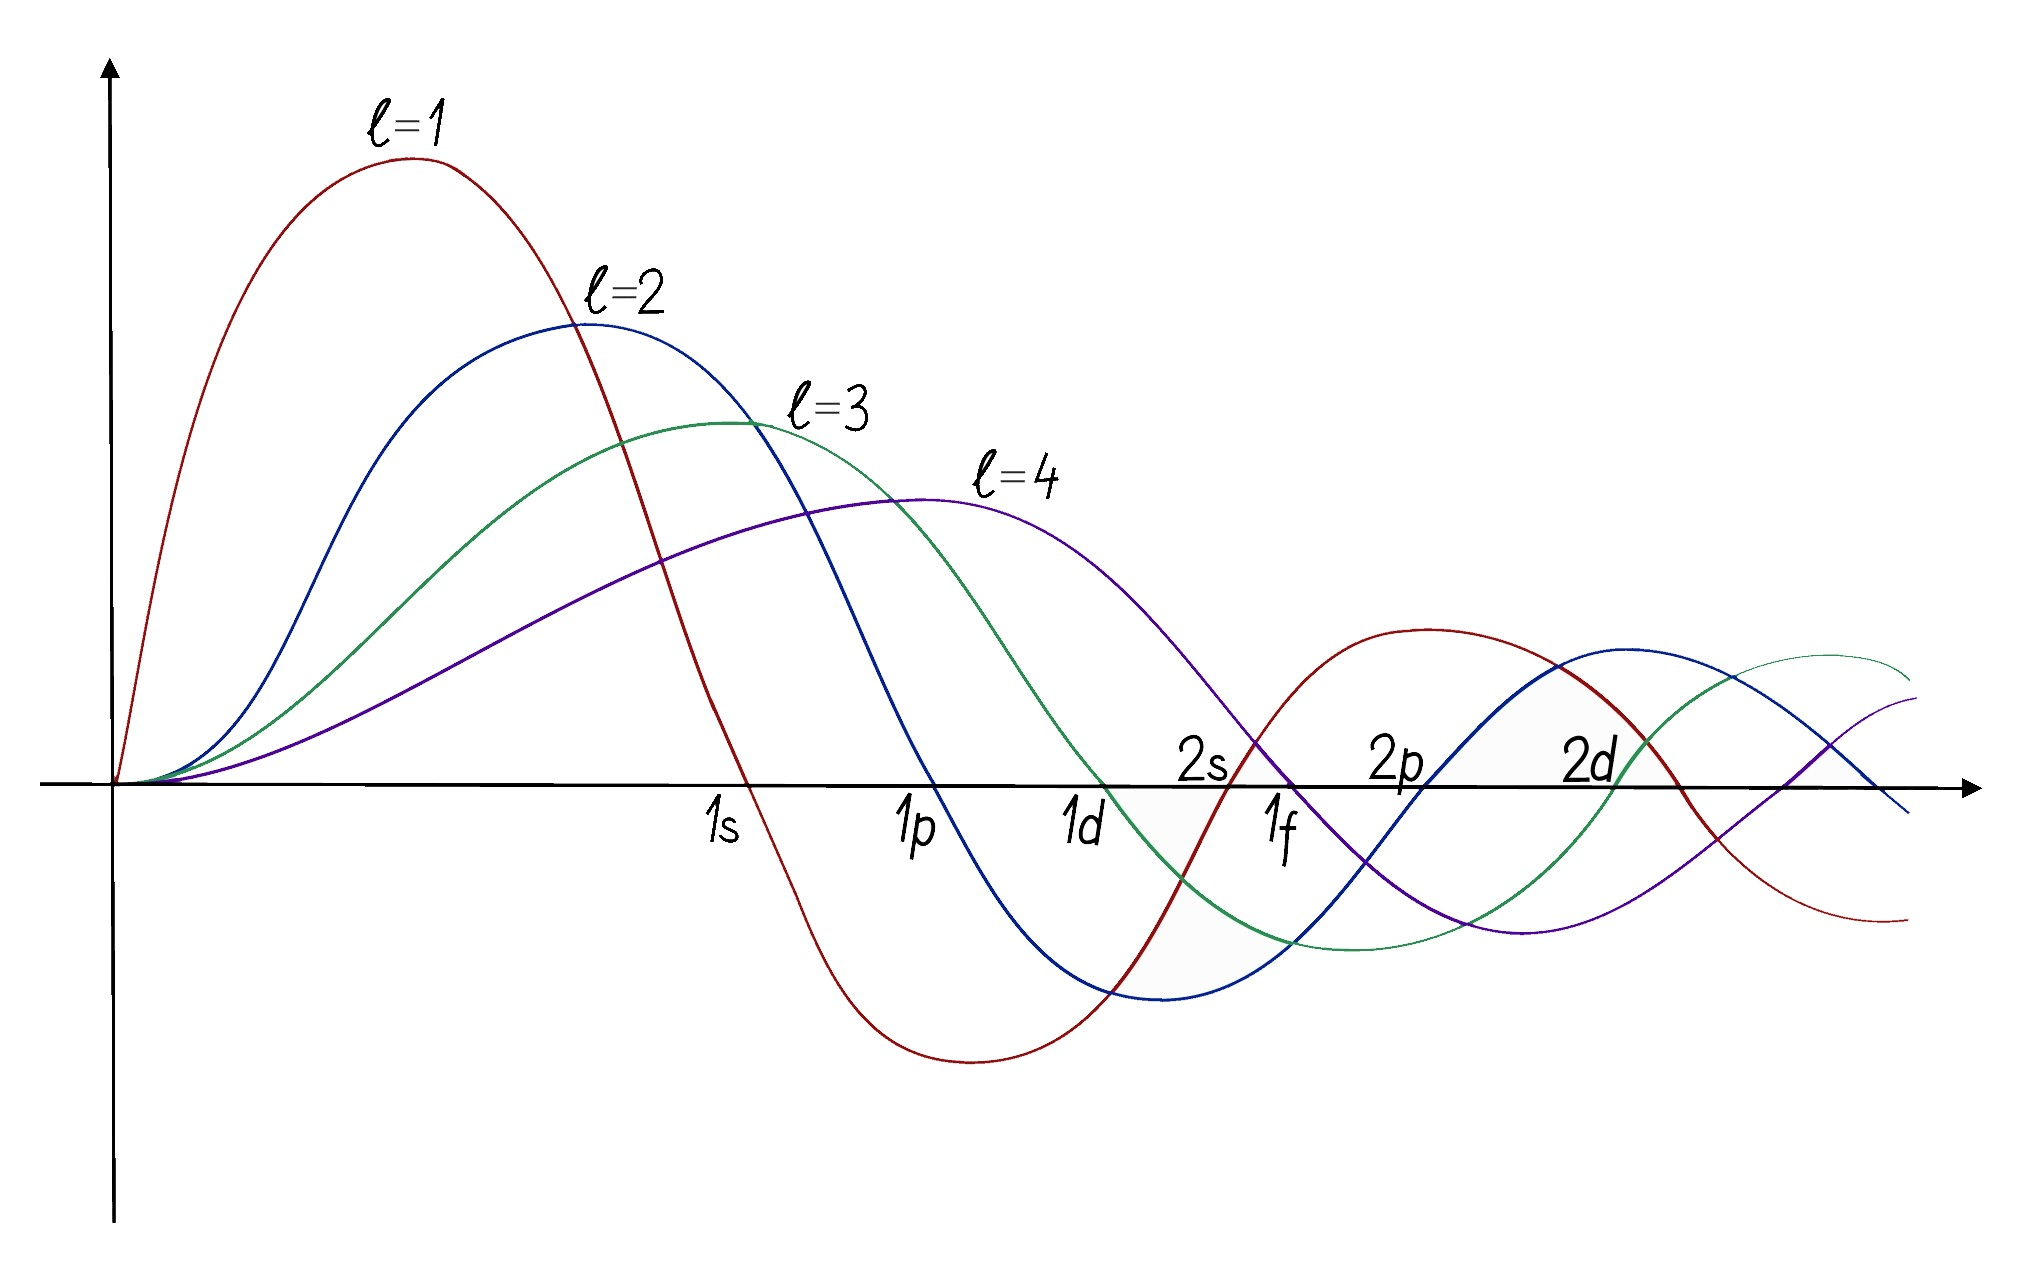
\includegraphics[scale=0.3]{class_10/images/bessel.jpg}
\caption{Первые сферические функции Бесселя}
\label{fig 10.1}
\end{figure}

\csquare{darklavender}


\excersize{Упражнение №34}{darklavender}
\begin{center}
    \textit{Электрон покоится в осциллирующем магнитном поле, направленном вдоль оси z:}
    \[
    \mathbf{B} = B_0\cos(\omega t)\hat{z}.
    \]
    \textit{Пусть в момент $t_0 = 0$ электрон со спином, направленным вдоль оси $x$, начинает движение. Определите положение спина (спинор) $\chi(t)$ в произвольный момент времени. Найдите вероятность получить $-\hbar/2$ при измерении спина по оси $x$ (то есть применяя оператор $\hat{S}_x$). Найдите минимальное поле $B_0$ необходимое для полного поворота спина в сторону против оси $x$.}
\end{center}

Для начала, немного теории. У частиц со спином есть так называемый собственный магнитный момент, который обозначается как $\boldsymbol{\mu}$. Эта величина зависит от спинового момента $\mathbf{S}$ следующим образом:
\[
\boldsymbol{\mu} = \gamma \mathbf{S}, \text{ где $\gamma$ - это гиромагнитное отношение.}
\]
Когда частица со спином помещается в магнитное поле, она испытывает крутящий момент $\boldsymbol{\mu} \times \mathbf{B}$, который поворачивает её спин по полю. Энергию этого крутящего момента можно вычислить как:
\[
H = -\boldsymbol{\mu}\cdot\mathbf{B} = -\gamma\mathbf{B}\cdot\mathbf{S}
\]
Зная это, запишем гамильтониан для нашей задачи:
\[
H = -\gamma\mathbf{B}\cdot\mathbf{S} = -\gamma B_0\cos(\omega t) \hat{S}_z = -\frac{\gamma B_0\hbar}{2}\cos(\omega t)\begin{pmatrix} 1 & 0 \\ 0 & -1 \end{pmatrix}
\]
Если забыли, откуда появилась такая матрица и что такое спин - вам в 8 семинар. 

Запишем спинор, определяющий положение спина на оси x:
\[
\chi(t) = \begin{pmatrix}\alpha(t)\\ \beta(t)\end{pmatrix}, \; \alpha(0) = \beta(0) = \frac{1}{\sqrt{2}}
\]
Теперь, чтобы получить значения $\alpha$ и $\beta$ в произвольный момент времени, решим уравнение Шрёдингера для спинора:
\begin{gather*}
i\hbar\frac{d\chi(t)}{dt} = H\chi(t) = -\frac{\gamma B_0\hbar}{2}\cos(\omega t)\begin{pmatrix} 1 & 0 \\ 0 & -1 \end{pmatrix}\begin{pmatrix}\alpha\\ \beta\end{pmatrix} =  -\frac{\gamma B_0\hbar}{2}\cos(\omega t) \begin{pmatrix} \alpha \\ -\beta \end{pmatrix} \implies \\
\implies i\hbar\begin{pmatrix} \dot{\alpha}\\ \dot{\beta} \end{pmatrix} = -\frac{\gamma B_0\hbar}{2}\cos(\omega t) \begin{pmatrix} \alpha \\ -\beta \end{pmatrix}
\end{gather*}
Решаем эту систему диффуров:
\begin{align*}
    \dot{\alpha} = i\frac{\gamma B_0}{2}\cos(\omega t)\alpha &\implies \frac{d\alpha}{\alpha} = i\frac{\gamma B_0}{2}\cos(\omega t)dt \implies \ln\alpha = i\frac{\gamma B_0}{2}\frac{\sin(\omega t)}{\omega} + C \implies \\ 
    & \implies \alpha(t) = Ae^{i\frac{\gamma B_0}{2\omega}\sin(\omega t)};\; \alpha(0) = A = \frac{1}{\sqrt{2}} \implies \\
    & \implies \alpha(t) = \frac{1}{\sqrt{2}}e^{i\frac{\gamma B_0}{2\omega}\sin(\omega t)}
\end{align*}
Аналогично для коэффициента $\beta$:
\[
\beta(t) = \frac{1}{\sqrt{2}}e^{-i\frac{\gamma B_0}{2\omega}\sin(\omega t)}
\]
Тогда
\begin{align*}
\chi(t) = \frac{1}{\sqrt{2}}\begin{pmatrix} e^{i\frac{\gamma B_0}{2\omega}\sin(\omega t)} \\ e^{-i\frac{\gamma B_0}{2\omega}\sin(\omega t)} \end{pmatrix}
\end{align*}

Найдём вероятность того, что спин частицы будет повернут антипараллельно оси x. Для этого воспользуемся правилом Борна:
\begin{align*}
P(\chi^{(x)}_-) &= \left|\bra{\chi^{(x)}_-}\ket{\chi(t)}\right|^2 = \left|(\frac{1}{\sqrt{2}})^2\begin{pmatrix}1 & -1\end{pmatrix}\begin{pmatrix} e^{i\frac{\gamma B_0}{2\omega}\sin(\omega t)} \\ e^{-i\frac{\gamma B_0}{2\omega}\sin(\omega t)} \end{pmatrix}\right|^2 = \\ &= \left|\frac{1}{2}(e^{i\frac{\gamma B_0}{2\omega}\sin(\omega t)} - e^{-i\frac{\gamma B_0}{2\omega}\sin(\omega t)})\right|^2 = \left|i\sin(\frac{\gamma B_0}{2\omega}\sin(\omega t))\right|^2 = \\
 & = \sin^2\left(\frac{\gamma B_0}{2\omega}\sin(\omega t)\right)
\end{align*}

Чтобы спин частицы развернулся в другую сторону, необходимо, чтобы $P(\chi^{(x)}_-) = 1$, то есть
\[
\sin^2\left(\frac{\gamma B_0}{2\omega}\sin(\omega t)\right) = 1 \implies \frac{\gamma B_0}{2\omega} = \frac{\pi}{2} \implies B_0 = \frac{\pi\omega}{\gamma}
\]

\csquare{darklavender}